\documentclass[preprint,12pt,authoryear]{elsarticle}
% Two-column Automatica layout: \documentclass[5p,twocolumn,authoryear]{elsarticle}

\usepackage{amsmath,amssymb,amsthm}
\usepackage{graphicx}
\usepackage{xcolor}
\usepackage{booktabs}
\graphicspath{{figures/}}
\usepackage{enumitem}
\usepackage{hyperref}

\newtheorem{theorem}{Theorem}
\newtheorem{proposition}[theorem]{Proposition}
\newtheorem{lemma}[theorem]{Lemma}
\newtheorem{corollary}[theorem]{Corollary}
\theoremstyle{definition}
\newtheorem{definition}[theorem]{Definition}
\newtheorem{assumption}{Assumption}
\newtheorem{problem}{Open problem}
\theoremstyle{remark}
\newtheorem{remark}[theorem]{Remark}

\newcommand{\R}{\mathbb{R}}
\newcommand{\N}{\mathbb{N}}
\newcommand{\Jet}{\mathcal{J}}
\newcommand{\tr}{^{\top}}
\newcommand{\PP}{\mathcal{P}}
\newcommand{\DD}{\mathcal{D}}
\newcommand{\NN}{\mathcal{N}}
\newcommand{\KK}{\mathcal{K}}
\newcommand{\Sol}{\mathcal{S}}
\newcommand{\dz}{\operatorname{dz}}
\newcommand{\sat}{\operatorname{sat}}
\DeclareMathOperator{\He}{He}
\DeclareMathOperator{\col}{col}
\DeclareMathOperator{\co}{co}
\DeclareMathOperator{\diag}{diag}
\DeclareMathOperator{\spn}{span}

\journal{Automatica}

\begin{document}
\begin{frontmatter}

\title{Lyapunov functions on jets of trajectories:\\ a universal quadratic form and converse results\tnoteref{t1}}
\tnotetext[t1]{\color{red}Working draft. This document was generated by Claude (Anthropic) in a dialogue with V.~Andrieu and S.~Tarbouriech, from a research question they posed; Y.~Ebihara joined the project afterwards; statements, proofs and numerical results have been read by the authors but not yet independently verified, and the references were cited from memory and must be checked.}

\author[lyon]{Vincent Andrieu}
\ead{vincent.andrieu@univ-lyon1.fr}
\author[kyushu]{Yoshio Ebihara}
\ead{ebihara@ees.kyushu-u.ac.jp}
\author[laas]{Sophie Tarbouriech}
\ead{tarbour@laas.fr}

\address[lyon]{Universit\'e Claude Bernard Lyon 1, CNRS, LAGEPP UMR 5007, 69100 Villeurbanne, France}
\address[kyushu]{Faculty of Information Science and Electrical Engineering, Kyushu University, Fukuoka 819-0395, Japan} % affiliation and e-mail to be confirmed
\address[laas]{LAAS-CNRS, Universit\'e de Toulouse, CNRS, 31400 Toulouse, France}

\begin{abstract}
Linear matrix inequality conditions for stability are often written with Lyapunov functions that are quadratic in an augmented vector such as $(x,\dot x)$ or $(x,\dot x,w,\dot w)$ rather than in the state $x$ alone. We formalize this practice by considering Lyapunov functions defined on the $N$-jet $(x,\dot x,\dots,x^{(N)})$ of the trajectories, with positivity and decrease required only on the jets that the system can generate. The main result is a converse theorem for uncertain linear systems: for any compact set of Hurwitz matrices there exist a horizon $T$ and an order $N$ such that a single quadratic form, whose coefficients do not depend on the set, is a common Lyapunov function on $N$-jets. This form is the finite-horizon energy of the Taylor prediction of the trajectory, and its time derivative obeys an identity that does not depend on the system. We derive from it an asymptotically exact hierarchy of LMI conditions for polytopic uncertainty, an explicit tolerance to slowly time-varying parameters, and a semi-global converse theorem for families of analytic nonlinear systems in which the order of the jet is dictated by the overshoot of the trajectories and by the radius of convergence of the Lie series. Systems with sector- and slope-restricted nonlinearities and systems with saturating actuators are then considered: for the latter, the order of the jet is limited to one by the piecewise-affine nature of the nonlinearity, and the corresponding piecewise-quadratic estimates of the region of attraction are computed by region-wise LMI conditions. Numerical examples illustrate the results.
\end{abstract}

\begin{keyword}
Lyapunov methods \sep robust stability \sep linear matrix inequalities \sep parameter-dependent Lyapunov functions \sep converse theorems \sep saturation
\end{keyword}
\end{frontmatter}

\section{Introduction}

\subsection{Motivation}
In the analysis of uncertain or nonlinear systems by linear matrix inequalities (LMIs), the Lyapunov function is frequently a quadratic form in an augmented vector. For a linear system $\dot x=Ax$, the form $V=\xi\tr\PP\xi$ with $\xi=(x,\dot x)$ leads, through Finsler's lemma and a slack variable, to conditions that are affine in $A$ and hence amenable to vertex tests over polytopes \citep{OliveiraSkelton2001,EbiharaBook2015}; higher-order derivatives of the state have been used in the same spirit to reduce conservatism \citep{Ebihara2005}. For Lur'e systems $\dot x=Ax+Bw$, $w=-\phi(Cx)$, with a sector- and slope-restricted nonlinearity, the augmented vector is $(x,\dot x,w,\dot w)$, and the sector and slope bounds become quadratic constraints on this vector handled by the S-procedure \citep{Park2002,Drummond2018}. For systems with saturating actuators, the generalized sector condition and the certified inclusion of a level set in the region where it holds follow the same pattern with the vector $(x,\dz(Kx))$ \citep{GomesdaSilva2005,TarbouriechPrieur2006,TarbouriechBook2011}.

In all these situations, the Lyapunov function is defined on a finite \emph{jet} of the trajectory, namely the value of $x$ and of its first derivatives at time $t$. The purpose of this paper is to develop a theory of Lyapunov functions on jets and to establish converse results that justify this practice.

\subsection{What jets do and do not bring}
For a deterministic system $\dot x=f(x)$, the $N$-jet of a trajectory is a function of the state, $x^{(k)}=L_f^kx$, and a function of the jet is a function of the state. What is gained is a \emph{linear parametrization}: a quadratic form in the jet, $\sum_{i,j\le N}(L_f^ix)\tr P_{ij}L_f^jx$, is a non-quadratic function of $x$ that depends linearly on the matrix $\PP=(P_{ij})$. The situation changes for uncertain systems $\dot x=f(x,w)$: the jet then depends on the unknown $w$, and a single quadratic form on jets generates a family of parameter-dependent Lyapunov functions with a fixed parametrization, whose size does not depend on the number of uncertain parameters. The temporal regularity of the uncertainty becomes decisive: if $w(t)$ can jump, so does $\dot x$, and a function of $(x,\dot x)$ cannot decrease along trajectories. Jets are therefore the natural tool for constant or slowly varying uncertainties, in the same way that Popov's criterion improves on the circle criterion for time-invariant nonlinearities and that rate-bounded parameter-dependent Lyapunov functions improve on quadratic stability \citep{Gahinet1996}.

\subsection{Contributions}
\begin{enumerate}[nosep,label=(\roman*)]
\item We define Lyapunov functions on jets, with positivity and decrease required only on the set of \emph{admissible} jets, and state the corresponding LMI conditions (Section~\ref{sec:jets}).
\item We introduce a \emph{universal} quadratic form $V_{T,N}$, the finite-horizon energy of the order-$N$ Taylor prediction of the trajectory, and prove an identity for its time derivative along any smooth curve (Section~\ref{sec:universal}). Theorem~\ref{thm:LTI} is a converse theorem with explicit constants: for any compact set of Hurwitz matrices, $V_{T,N}$ is a common Lyapunov function on $N$-jets for suitable $T$ and $N$.
\item For polytopic uncertainty we obtain a nested hierarchy of LMI conditions that is asymptotically exact (Section~\ref{sec:polytope}).
\item For time-varying parameters we prove that the same forms tolerate an explicit rate bound and yield parameter-dependent Lyapunov functions whose rate tolerance does not degrade with the order (Section~\ref{sec:tv}).
\item For families of analytic nonlinear systems we prove a semi-global converse theorem in which the order of the jet is governed by the overshoot time and by the radius of convergence of the Lie series (Section~\ref{sec:NL}).
\item We treat sector- and slope-restricted Lur'e systems and exhibit a conserved quantity of the associated parameter-varying system (Section~\ref{sec:lure}).
\item We show how the framework adapts to the regional analysis of saturated systems: the order of the jet is limited to one, the corresponding functions are piecewise quadratic, and region-wise LMI conditions provide non-ellipsoidal estimates of the region of attraction (Section~\ref{sec:regional}).
\end{enumerate}
Numerical illustrations are gathered in Section~\ref{sec:num}, and open problems in Section~\ref{sec:conc}.

\subsection{Related work}
For a single linear time-invariant system, quadratic forms in the jet are the \emph{quadratic differential forms} of \citet{WillemsTrentelman1998}, and the derivative identity of Section~\ref{sec:universal} has a natural expression in their two-variable polynomial calculus; see \citet{KojimaTakaba2005} for the discrete-time counterpart. Conditions involving higher-order derivatives of a Lyapunov function go back to \citet{Butz1969}, and non-monotonic Lyapunov functions were studied by \citet{AhmadiParrilo2008}. Parameter-dependent Lyapunov functions with affine or polynomial dependence and their P\'olya-type relaxations are treated in \citet{Gahinet1996,Chesi2005,OliveiraPeres2007,Scherer2005}. The projection of a finite window of the trajectory on an orthogonal basis is at the heart of the Bessel--Legendre hierarchies for time-delay systems \citep{SeuretGouaisbaut2015}, whose necessity was established by \citet{Bajodek2023}; the present work can be seen as the ``future'' counterpart of their ``past'' window. In discrete time, Lyapunov functions on finite windows of the trajectory underlie the approximations of the joint spectral radius and the path-complete Lyapunov functions of \citet{Ahmadi2014}. Krasovskii's method $V=f\tr Pf$ \citep{Krasovskii1963} and Finsler--Lyapunov functions for contraction \citep{ForniSepulchre2014,AndrieuJP2016} are Lyapunov functions on $1$-jets with state-dependent weights. Piecewise-quadratic Lyapunov functions for saturated systems built on $(x,\dz(Kx))$ were introduced by \citet{Dai2009}, following the piecewise-quadratic constructions of \citet{JohanssonRantzer1998}. Finally, the analytic nonlinear part connects with the Koopman-operator approach to stability \citep{MauroyMezic2016} and with the existence of polynomial Lyapunov functions on compact sets \citep{Peet2009}.

\subsection{Notation}
$|\cdot|$ is the Euclidean norm and $\|\cdot\|$ the induced matrix norm; $I$ is the identity. $\He(M)=M+M\tr$. For $A\in\R^{n\times n}$ and $N\in\N$, $\Gamma_N(A)=\col(I,A,\dots,A^N)\in\R^{n(N+1)\times n}$ and $E_N(M)=\sum_{k=0}^NM^k/k!$. $\Delta_m$ is the unit simplex of $\R^m$. A function $\alpha:\R_{\ge0}\to\R_{\ge0}$ is of class $\mathcal K_\infty$ if it is continuous, increasing, unbounded and $\alpha(0)=0$; $\beta:\R_{\ge0}^2\to\R_{\ge0}$ is of class $\mathcal{KL}$ if $\beta(\cdot,t)\in\mathcal K_\infty$ for each $t$ and $\beta(s,\cdot)$ decreases to $0$ for each $s$. For a $C^1$ function $V$ on $\R^{p}$, $DV(j)[h]$ denotes its derivative at $j$ in the direction $h$. Elements of $\R^{n(N+1)}$ (jets of order $N$) are written $j=(x_0,\dots,x_N)$ and elements of $\R^{n(N+2)}$ (jets of order $N+1$) are written $\bar j=(x_0,\dots,x_{N+1})$; the two linear maps
\begin{equation}\label{eq:pisigma}
\pi(\bar j):=(x_0,\dots,x_N),\qquad \sigma(\bar j):=(x_1,\dots,x_{N+1}),
\end{equation}
are the \emph{truncation} and the \emph{shift}, and the same symbols denote their matrices. $E_0j=x_0$ and $\bar E_0\bar j=x_0$ are the projections on the base point.

\section{Lyapunov functions on jets}\label{sec:jets}

\subsection{Systems and admissible jets}
A system $\Sigma$ is described by a set $\Sol$ of solutions $x:[0,\infty)\to\R^n$, each of class $C^{N+1}$. This covers $\dot x=f(x)$ with $f\in C^N$, $\dot x=f(x,w)$ with $w$ constant in a set $W$ or $w(\cdot)$ of class $C^N$, and Lur'e systems with $\phi\in C^N$. The $N$-jet of a solution at time $t$ is
\begin{equation}\label{eq:jet}
j^Nx(t):=\big(x(t),\dot x(t),\dots,x^{(N)}(t)\big)\in\R^{n(N+1)},
\end{equation}
and the set of \emph{admissible $N$-jets} of $\Sigma$ is
\begin{equation}\label{eq:adm}
\Jet^N_\Sigma:=\big\{j^Nx(t)\ :\ x\in\Sol,\ t\ge0\big\}.
\end{equation}
With the truncation and shift maps \eqref{eq:pisigma},
\begin{equation}\label{eq:shift}
j^Nx(t)=\pi\big(j^{N+1}x(t)\big),\qquad \frac{d}{dt}j^Nx(t)=\sigma\big(j^{N+1}x(t)\big).
\end{equation}

\subsection{Definition and basic property}
\begin{definition}\label{def:jetLF}
A function $V\in C^1(\R^{n(N+1)},\R)$ is a \emph{Lyapunov function on $N$-jets} for $\Sigma$ if there exist $\alpha_1,\alpha_2,\alpha_3\in\mathcal K_\infty$ such that
\begin{align}
\alpha_1(|x_0|)\le V(j)\le\alpha_2(|x_0|)\qquad&\forall j=(x_0,\dots,x_N)\in\Jet^N_\Sigma,\label{eq:pos}\\
DV\big(\pi(\bar j)\big)\big[\sigma(\bar j)\big]\le-\alpha_3(|x_0|)\qquad&\forall \bar j=(x_0,\dots,x_{N+1})\in\Jet^{N+1}_\Sigma.\label{eq:dec}
\end{align}
\end{definition}
Both conditions are only required on admissible jets. By \eqref{eq:shift}, the left-hand side of \eqref{eq:dec} is $\frac{d}{dt}V(j^Nx(t))$ along solutions.

\begin{proposition}\label{prop:stab}
If $V$ is a Lyapunov function on $N$-jets for $\Sigma$, there exists $\beta\in\mathcal{KL}$ such that $|x(t)|\le\beta(|x(0)|,t)$ for every $x\in\Sol$ and $t\ge0$.
\end{proposition}
\begin{proof}
Let $x\in\Sol$ and $v(t)=V(j^Nx(t))$, a $C^1$ function. By \eqref{eq:pos}, \eqref{eq:dec} and \eqref{eq:shift},
\begin{equation}\label{eq:comp}
\alpha_1(|x(t)|)\le v(t)\le\alpha_2(|x(t)|),\qquad \dot v(t)\le-\alpha_3(|x(t)|)\le-\alpha_3\circ\alpha_2^{-1}(v(t)).
\end{equation}
By the comparison lemma \citep[Lemma 4.4]{Khalil2002}, there exists $\gamma\in\mathcal{KL}$, depending only on $\alpha_3\circ\alpha_2^{-1}$, such that $v(t)\le\gamma(v(0),t)$. Hence $|x(t)|\le\alpha_1^{-1}\big(\gamma(\alpha_2(|x(0)|),t)\big)=:\beta(|x(0)|,t)$.
\end{proof}

\begin{remark}[deterministic systems]\label{rem:det}
If $\Sol$ is the set of solutions of $\dot x=f(x)$, $f\in C^N$, then $j^Nx(t)=\Phi_N(x(t))$ with $\Phi_N(x)=(x,L_fx,\dots,L_f^Nx)$, and $V$ is a Lyapunov function on $N$-jets if and only if $V\circ\Phi_N$ is a Lyapunov function. Since every Lyapunov function is a function of the $0$-jet, converse questions are only meaningful relative to a class of functions of the jet. For quadratic forms $V(j)=j\tr\PP j$, the class of the functions $V\circ\Phi_N$ is
\begin{equation}\label{eq:QN}
\mathcal Q_N(f):=\Big\{x\mapsto\sum_{i,j=0}^N(L_f^ix)\tr P_{ij}\,L_f^jx\ :\ P_{ij}\in\R^{n\times n}\Big\}.
\end{equation}
\end{remark}

\subsection{Quadratic forms and LMI conditions}
Let $V(j)=j\tr\PP j$ with $\PP=\PP\tr\in\R^{n(N+1)\times n(N+1)}$. The left-hand side of \eqref{eq:dec} is $2\,\pi(\bar j)\tr\PP\,\sigma(\bar j)=\bar j\tr\DD(\PP)\bar j$ with
\begin{equation}\label{eq:D}
\DD(\PP):=\He\big(\pi\tr\PP\,\sigma\big),
\end{equation}
a linear function of $\PP$. Suppose that the admissible jets satisfy, for some $w$ in a set $W$, the equality constraints $\NN_0(w)j=0$, $\NN(w)\bar j=0$ and the quadratic constraints $j\tr\Theta^0_\ell(w)j\ge0$, $\bar j\tr\Theta_\ell(w)\bar j\ge0$, $\ell=1,\dots,L$.
\begin{proposition}\label{prop:LMI}
Assume that $|j|\le\kappa(|x_0|)$ on $\Jet^N_\Sigma$ for some $\kappa\in\mathcal K_\infty$. If there exist $\PP$, matrices $G_0,G_1$, scalars $\mu_\ell,\lambda_\ell\ge0$ and $\varepsilon>0$ such that, for all $w\in W$,
\begin{align}
\PP+\He\big(G_0\NN_0(w)\big)-\sum_{\ell=1}^L\mu_\ell\Theta^0_\ell(w)&\succeq\varepsilon E_0\tr E_0,\label{eq:LMIpos}\\
\DD(\PP)+\He\big(G_1\NN(w)\big)+\sum_{\ell=1}^L\lambda_\ell\Theta_\ell(w)&\preceq-\varepsilon \bar E_0\tr\bar E_0,\label{eq:LMIdec}
\end{align}
then $V$ is a Lyapunov function on $N$-jets for $\Sigma$.
\end{proposition}
\begin{proof}
Let $j\in\Jet^N_\Sigma$ and let $w$ be the corresponding uncertainty. Multiplying \eqref{eq:LMIpos} on the left by $j\tr$ and on the right by $j$, and using $\NN_0(w)j=0$ and $j\tr\Theta^0_\ell(w)j\ge0$,
\begin{equation}
V(j)\ \ge\ \varepsilon|x_0|^2+\sum_{\ell=1}^L\mu_\ell\,j\tr\Theta^0_\ell(w)j\ \ge\ \varepsilon|x_0|^2 ,
\end{equation}
and $V(j)\le\|\PP\|\kappa(|x_0|)^2$. Likewise, \eqref{eq:LMIdec} gives $\bar j\tr\DD(\PP)\bar j\le-\varepsilon|x_0|^2$ on $\Jet^{N+1}_\Sigma$.
\end{proof}
When $\NN_0,\NN$ are affine in $w$ and $G_0,G_1,\mu_\ell,\lambda_\ell$ do not depend on $w$, \eqref{eq:LMIpos}--\eqref{eq:LMIdec} are affine in $w$ and reduce, for polytopic $W$, to finitely many LMIs at the vertices.

\section{A universal quadratic form}\label{sec:universal}

\subsection{Definition}
For a curve $x(\cdot)$ of class $C^{N+1}$ and $t\ge0$, let
\begin{equation}\label{eq:taylor}
\tau_N(s):=\sum_{k=0}^N\frac{s^k}{k!}\,x^{(k)}(t),\qquad s\in\R,
\end{equation}
be the order-$N$ Taylor prediction of the trajectory from time $t$; it is a linear function of $j^Nx(t)$. For $T>0$ we define
\begin{equation}\label{eq:VTN}\hspace*{-1em}
V_{T,N}(j^Nx):=\int_0^T|\tau_N(s)|^2ds=\sum_{i,j=0}^Nh_{ij}(T)\,(x^{(i)})\tr x^{(j)},\quad h_{ij}(T):=\frac{T^{i+j+1}}{(i+j+1)\,i!\,j!}\,,
\end{equation}
which is a quadratic form in $j^Nx$.
Indeed, $V_{T,N}(j)=j\tr(H_{T,N}\otimes I)j$, where $H_{T,N}=(h_{ij}(T))_{i,j\le N}$ is the Gram matrix of the functions $s^k/k!$, $k=0,\dots,N$, in $L^2[0,T]$. In particular $H_{T,N}\succ0$ and $V_{T,N}$ is positive definite on the whole jet space; only the decrease condition depends on the system. The coefficients $h_{ij}(T)$ do not depend on the system either.

\subsection{The derivative identity}
\begin{lemma}\label{lem:dV}
For every curve $x(\cdot)$ of class $C^{N+1}$ and every $t\ge0$,
\begin{equation}\label{eq:dVTN}
\frac{d}{dt}V_{T,N}\big(j^Nx(t)\big)=|\tau_N(T)|^2-|x(t)|^2+\frac{2}{N!}\int_0^Ts^N\,\tau_N(s)\tr x^{(N+1)}(t)\,ds .
\end{equation}
\end{lemma}
\begin{proof}
From \eqref{eq:taylor},
\begin{align}\label{eq:dtau}
\frac{d}{dt}\tau_N(s)=\sum_{k=0}^N\frac{s^k}{k!}x^{(k+1)}(t)&=\sum_{k=1}^{N}\frac{s^{k-1}}{(k-1)!}x^{(k)}(t)+\frac{s^N}{N!}x^{(N+1)}(t)\nonumber\\
&=\partial_s\tau_N(s)+\frac{s^N}{N!}x^{(N+1)}(t).
\end{align}
Hence
\begin{equation}
\frac{d}{dt}\int_0^T|\tau_N(s)|^2ds=\int_0^T\partial_s|\tau_N(s)|^2ds+\frac{2}{N!}\int_0^Ts^N\tau_N(s)\tr x^{(N+1)}(t)ds ,
\end{equation}
and $\int_0^T\partial_s|\tau_N(s)|^2ds=|\tau_N(T)|^2-|\tau_N(0)|^2$ with $\tau_N(0)=x(t)$.
\end{proof}
Identity \eqref{eq:dVTN} decomposes the derivative into $-|x|^2$, the squared prediction at the horizon, and a truncation error. It holds for any curve: the system enters only through the set of admissible jets. In the two-variable calculus of \citet{WillemsTrentelman1998}, the limit $N\to\infty$ corresponds to the entire function $\Phi_T(\zeta,\eta)=\int_0^Te^{s(\zeta+\eta)}ds$, for which $(\zeta+\eta)\Phi_T(\zeta,\eta)=e^{T(\zeta+\eta)}-1$, that is, $\frac{d}{dt}\int_0^T|x(t+s)|^2ds=|x(t+T)|^2-|x(t)|^2$.

\subsection{Converse theorem for compact families of linear systems}
\begin{lemma}\label{lem:unif}
Let $\KK\subset\R^{n\times n}$ be a compact set of Hurwitz matrices. There exist $c\ge1$ and $\lambda>0$ such that
\begin{equation}\label{eq:unif}
\|e^{At}\|\le c\,e^{-\lambda t}\qquad\forall A\in\KK,\ \forall t\ge0 .
\end{equation}
\end{lemma}
\begin{proof}
The map $A\mapsto P(A)$, where $P(A)$ is the solution of $A\tr P+PA=-I$, is continuous on the open set of Hurwitz matrices. By compactness, there are $0<p_1\le p_2$ with $p_1I\preceq P(A)\preceq p_2I$ for all $A\in\KK$. Along $\dot x=Ax$,
\begin{equation}
\frac{d}{dt}\,x\tr P(A)x=-|x|^2\le-\frac1{p_2}\,x\tr P(A)x,\qquad\text{hence}\qquad p_1|e^{At}x|^2\le e^{-t/p_2}p_2|x|^2 ,
\end{equation}
which is \eqref{eq:unif} with $c=\sqrt{p_2/p_1}$ and $\lambda=1/(2p_2)$.
\end{proof}

\begin{theorem}\label{thm:LTI}
Let $\KK\subset\R^{n\times n}$ be a compact set of Hurwitz matrices, let $c,\lambda$ satisfy \eqref{eq:unif}, and let $a:=\max_{A\in\KK}\|A\|$. Let $T>0$ and $N\in\N$ satisfy
\begin{equation}\label{eq:TN}
c^2e^{-2\lambda T}\ \le\ \frac12,\qquad e^{2Ta}\,\frac{(Ta)^{N+1}}{(N+1)!}\ \le\ \frac{1}{16}.
\end{equation}
Then, for every $A\in\KK$ and every solution of $\dot x=Ax$,
\begin{equation}\label{eq:concl}
V_{T,N}(j^Nx)\ \ge\ \frac{1-e^{-2aT}}{4a}\,|x|^2,\qquad \frac{d}{dt}V_{T,N}(j^Nx)\ \le\ -\frac14|x|^2 .
\end{equation}
The first condition in \eqref{eq:TN} holds for $T\ge\ln(2c^2)/(2\lambda)$ and the second one for $N\ge e^2Ta+2$.
Consequently, $V_{T,N}$ is a common Lyapunov function on $N$-jets for the family $\{\dot x=Ax:A\in\KK\}$, and
\begin{equation}\label{eq:PTN}
x\tr P_{T,N}(A)x,\qquad P_{T,N}(A):=\Gamma_N(A)\tr(H_{T,N}\otimes I)\Gamma_N(A)=\sum_{i,j=0}^Nh_{ij}(T)\,(A\tr)^iA^j,
\end{equation}
is a parameter-dependent Lyapunov function, polynomial of degree $2N$ in $A$.
\end{theorem}
\begin{proof}
Along $\dot x=Ax$, $x^{(k)}=A^kx$, hence $\tau_N(s)=E_N(sA)x$ and $x^{(N+1)}=A^{N+1}x$. By Lemma~\ref{lem:dV}, $\frac{d}{dt}V_{T,N}=x\tr M_{T,N}(A)x$ with
\begin{equation}\label{eq:M}
M_{T,N}(A):=E_N(TA)\tr E_N(TA)-I+\frac{1}{N!}\He\Big(\int_0^Ts^NE_N(sA)\tr ds\;A^{N+1}\Big).
\end{equation}
Let $\epsilon_N:=\sum_{k>N}(Ta)^k/k!$. Since $\|E_N(sA)\|\le e^{sa}$ for $s\in[0,T]$ and $\|e^{TA}-E_N(TA)\|\le\epsilon_N$,
\begin{align}
\|E_N(TA)\tr E_N(TA)-e^{TA\tr}e^{TA}\|&\le\|E_N(TA)-e^{TA}\|\big(\|E_N(TA)\|+\|e^{TA}\|\big)\nonumber\\&\le2e^{Ta}\epsilon_N,\label{eq:b1}\\
\Big\|\frac{1}{N!}\He\Big(\int_0^Ts^NE_N(sA)\tr ds\,A^{N+1}\Big)\Big\|&\le\frac{2}{N!}\int_0^Ts^Ne^{sa}ds\;a^{N+1}\le2e^{Ta}\frac{(Ta)^{N+1}}{(N+1)!}.\label{eq:b2}
\end{align}
Moreover, $\epsilon_N\le\frac{(Ta)^{N+1}}{(N+1)!}\sum_{k\ge0}\frac{(Ta)^k}{k!}=\frac{(Ta)^{N+1}}{(N+1)!}e^{Ta}$. Combining \eqref{eq:b1}, \eqref{eq:b2} and the second condition in \eqref{eq:TN},
\begin{equation}\label{eq:b3}
\big\|M_{T,N}(A)-\big(e^{TA\tr}e^{TA}-I\big)\big\|\le2e^{Ta}\frac{(Ta)^{N+1}}{(N+1)!}\big(e^{Ta}+1\big)\le4e^{2Ta}\frac{(Ta)^{N+1}}{(N+1)!}\le\frac14 .
\end{equation}
By \eqref{eq:unif} and the first condition in \eqref{eq:TN}, $e^{TA\tr}e^{TA}-I\preceq(c^2e^{-2\lambda T}-1)I\preceq-\frac12I$, and \eqref{eq:b3} yields $M_{T,N}(A)\preceq-\frac14I$, which is the second inequality in \eqref{eq:concl}. The sufficient condition $N\ge e^2Ta+2$ follows from $(N+1)!\ge((N+1)/e)^{N+1}$: if $N+1\ge e^2Ta$ then $\frac{(Ta)^{N+1}}{(N+1)!}\le\big(\frac{eTa}{N+1}\big)^{N+1}\le e^{-(N+1)}$, and $e^{-(N+1)}\le e^{-2Ta}/16$ as soon as $N+1\ge2Ta+\ln16$; both hold when $N+1\ge e^2Ta+3$.

For the first inequality, note that $|x|=|e^{-sA}e^{sA}x|\le e^{sa}|e^{sA}x|$, so that $|e^{sA}x|\ge e^{-sa}|x|$. By \eqref{eq:TN}, $\epsilon_N\le\frac{(Ta)^{N+1}}{(N+1)!}e^{Ta}\le\frac{1}{16}e^{-Ta}\le\frac1{16}e^{-sa}$ for $s\in[0,T]$. Hence
\begin{equation}
|E_N(sA)x|\ \ge\ |e^{sA}x|-\|e^{sA}-E_N(sA)\|\,|x|\ \ge\ \big(e^{-sa}-\epsilon_N\big)|x|\ \ge\ \frac{15}{16}e^{-sa}|x| ,
\end{equation}
and $V_{T,N}(j^Nx)=\int_0^T|E_N(sA)x|^2ds\ge\frac{225}{256}\int_0^Te^{-2sa}ds\,|x|^2\ge\frac{1-e^{-2aT}}{4a}|x|^2$. Finally, $V_{T,N}(j^Nx)\le\|H_{T,N}\|\,\|\Gamma_N(A)\|^2|x|^2$, so that Definition~\ref{def:jetLF} holds with quadratic bounds.
\end{proof}

\begin{remark}[interpretation]\label{rem:interp}
Theorem~\ref{thm:LTI} states that the truncation of the infinite-order Lyapunov function $V_T(x)=\int_0^T|x(t+s)|^2ds=x\tr P_T(A)x$, $P_T(A)=\int_0^Te^{A\tr s}e^{As}ds$, remains a common Lyapunov function once the order is large enough. The two conditions in \eqref{eq:TN} have a simple meaning: the horizon $T$ exceeds the time after which the norm has decreased by a factor $\sqrt2$ for every matrix of the family, and the Taylor remainder of $e^{TA}$ at order $N$, amplified by the worst-case factor $e^{2Ta}$, is small enough for $M_{T,N}(A)$ in \eqref{eq:M} to be within $\frac14$ of its limit $e^{TA\tr}e^{TA}-I$. With $T=\ln(2c^2)/(2\lambda)$, the order $N\ge e^2Ta+2$ is governed by the ratio $a/\lambda$ and by the logarithm of the overshoot $c$. The lower bound in \eqref{eq:concl} is half the energy on $[0,T]$ of a trajectory decaying at the fastest admissible rate $a$. These constants are conservative (see Section~\ref{sec:numpoly}): Theorem~\ref{thm:LTI} is an existence result, and the computational object is the LMI with free $\PP$ of Section~\ref{sec:polytope}. Weighted variants $\int_0^T\tau_N(s)\tr Q\tau_N(s)ds$ and, more generally, $\iint\tau_N(s)\tr K(s,s')\tau_N(s')\,ds\,ds'$ are also quadratic forms in the jet; the proof applies with $c$ replaced by the overshoot in the norm $|\cdot|_Q$.
\end{remark}

\begin{remark}[numerical basis]\label{rem:legendre}
With $D=\diag(T^k/k!)_{k\le N}$ and $\mathcal H_{N+1}=(1/(i+j+1))_{i,j\le N}$ the Hilbert matrix, $H_{T,N}=T\,D\mathcal H_{N+1}D$; its condition number exceeds $10^7$ for $N=4$ and $10^{18}$ for $N=8$ at $T=1$. In computations, $\tau_N$ should be expanded on the shifted Legendre polynomials of $[0,T]$, $\tau_N(s)=\sum_k\ell_k(s)z_k$ with $z=Mj$ for a fixed triangular $M$, so that $V_{T,N}=\sum_k|z_k|^2$. This is the change of basis underlying the hierarchies of \citet{SeuretGouaisbaut2015}.
\end{remark}

\begin{remark}[discrete time]
For $x_{t+1}=Ax_t$, the analogue of the $N$-jet is the window $(x_t,\dots,x_{t+N})$, and $V=\sum_{i\le N}|x_{t+i}|^2$ satisfies $V_{t+1}-V_t=|x_{t+N+1}|^2-|x_t|^2$. The common decrease condition is $\|A^{N+1}\|<1$ on $\KK$, which holds for $N$ large by the discrete counterpart of Lemma~\ref{lem:unif}; this is the classical $\ell$-step norm criterion \citep{Ahmadi2014}.
\end{remark}

\section{Polytopic uncertainty: an exact hierarchy}\label{sec:polytope}

Let $A(\alpha)=\sum_{i=1}^m\alpha_iA_i$, $\alpha\in\Delta_m$, and $\KK=\co\{A_1,\dots,A_m\}$. Along $\dot x=A(\alpha)x$, the admissible $N$-jets are $\Gamma_N(A(\alpha))x$, and the conditions of Definition~\ref{def:jetLF} for $V(j)=j\tr\PP j$ read
\begin{equation}\label{eq:robcond}
\Gamma_N(A(\alpha))\tr\PP\,\Gamma_N(A(\alpha))\succ0,\quad\Gamma_{N+1}(A(\alpha))\tr\DD(\PP)\,\Gamma_{N+1}(A(\alpha))\prec0,\quad\alpha\in\Delta_m .
\end{equation}
Let $\hat\Gamma_N(\alpha)$ denote the homogenization of $\Gamma_N(A(\alpha))$, obtained by multiplying its $k$-th block $A(\alpha)^k$ by $(\sum_i\alpha_i)^{N-k}$, and define the homogeneous matrix polynomials
\begin{equation}\label{eq:FQ}
Q_\PP(\alpha):=\hat\Gamma_N(\alpha)\tr\PP\hat\Gamma_N(\alpha)-\Big(\sum_i\alpha_i\Big)^{2N}I,\quad F_\PP(\alpha):=\hat\Gamma_{N+1}(\alpha)\tr\DD(\PP)\hat\Gamma_{N+1}(\alpha),
\end{equation}
of degrees $2N$ and $2N+2$, which coincide on $\Delta_m$ with the two matrices in \eqref{eq:robcond}, the first one shifted by $-I$. For $d\in\N$, let $\{Q^{(d)}_{\PP,\kappa}\}$ and $\{F^{(d)}_{\PP,\kappa}\}$ be the coefficient matrices of $(\sum_i\alpha_i)^dQ_\PP(\alpha)$ and $(\sum_i\alpha_i)^dF_\PP(\alpha)$; they depend linearly on $\PP$.

\begin{definition}[level $(N,d)$]
$\mathrm{LMI}(N,d)$: find $\PP=\PP\tr\in\R^{n(N+1)\times n(N+1)}$ such that
\begin{equation}\label{eq:LMINd}
Q^{(d)}_{\PP,\kappa}\succeq0\quad\forall\kappa,\ |\kappa|=2N+d,\qquad F^{(d)}_{\PP,\kappa}\prec0\quad\forall\kappa,\ |\kappa|=2N+2+d .
\end{equation}
\end{definition}

\begin{theorem}\label{thm:hier}
\begin{enumerate}[nosep,label=(\roman*)]
\item If $\mathrm{LMI}(N,d)$ is feasible, then $V(j)=j\tr\PP j$ is a common Lyapunov function on $N$-jets for $\{\dot x=Ax:A\in\KK\}$.
\item If $\mathrm{LMI}(N,d)$ is feasible, then $\mathrm{LMI}(N,d+1)$ and $\mathrm{LMI}(N+1,d)$ are feasible.
\item If $\KK$ is Hurwitz, then $\mathrm{LMI}(N,d)$ is feasible for some $(N,d)$.
\end{enumerate}
\end{theorem}
\begin{proof}
(i) For $\alpha\in\Delta_m$, all monomials $\alpha^\kappa$ are nonnegative and $(\sum_i\alpha_i)^p=1$ for every $p$, so that \eqref{eq:LMINd} implies $Q_\PP(\alpha)\succeq0$ and $F_\PP(\alpha)\prec0$, that is,
\begin{equation}
\Gamma_N(A(\alpha))\tr\PP\,\Gamma_N(A(\alpha))\succeq I,\quad\Gamma_{N+1}(A(\alpha))\tr\DD(\PP)\,\Gamma_{N+1}(A(\alpha))\prec0,\quad\alpha\in\Delta_m .
\end{equation}
By compactness of $\Delta_m$ there is $\varepsilon>0$ such that the second matrix is $\preceq-\varepsilon I$. Definition~\ref{def:jetLF} then holds with $\alpha_1(s)=s^2$, $\alpha_2(s)=\|\PP\|\max_{\alpha}\|\Gamma_N(A(\alpha))\|^2s^2$ and $\alpha_3(s)=\varepsilon s^2$.

(ii) Multiplying by $\sum_i\alpha_i$, each coefficient at level $d+1$ is a sum of coefficients at level $d$ and has the required sign. For $N+1$, let $\PP'=\diag(\PP,0)$. Then $\DD(\PP')=\diag(\DD(\PP),0)$ and
\begin{align}
\hat\Gamma_{N+1}(\alpha)\tr\PP'\hat\Gamma_{N+1}(\alpha)&=\Big(\sum_i\alpha_i\Big)^2\hat\Gamma_N(\alpha)\tr\PP\hat\Gamma_N(\alpha),\nonumber\\
\hat\Gamma_{N+2}(\alpha)\tr\DD(\PP')\hat\Gamma_{N+2}(\alpha)&=\Big(\sum_i\alpha_i\Big)^2F_\PP(\alpha),
\end{align}
so that the coefficients of level $(N+1,d)$ for $\PP'$ are those of level $(N,d+2)$ for $\PP$, which have the required sign by the first part.

(iii) Let $T,N$ satisfy \eqref{eq:TN} and $\PP_0=H_{T,N}\otimes I$. By \eqref{eq:concl}, there is $\varepsilon>0$ such that $\Gamma_N(A)\tr\PP_0\Gamma_N(A)\succeq\varepsilon I$ and $\Gamma_{N+1}(A)\tr\DD(\PP_0)\Gamma_{N+1}(A)\preceq-\frac14I$ for all $A\in\KK$. With $\PP=2\PP_0/\varepsilon$, the homogeneous matrix polynomials $Q_\PP$ and $-F_\PP$ are positive definite on $\Delta_m$. By P\'olya's theorem for matrix-valued polynomials \citep{Scherer2005,OliveiraPeres2007}, there is $d$ such that all coefficients of $(\sum_i\alpha_i)^dQ_\PP$ and of $-(\sum_i\alpha_i)^dF_\PP$ are positive definite.
\end{proof}

\begin{remark}[vertex conditions with slack variables]\label{rem:slack}
The practical counterpart of \eqref{eq:LMINd} is the Finsler form of Proposition~\ref{prop:LMI}. With $\NN_0(A)j=(x_{k+1}-Ax_k)_{k<N}$ and $\NN(A)\bar j=(x_{k+1}-Ax_k)_{k\le N}$, both affine in $A$, and constant multipliers $G_0,G$, one obtains the $m$ vertex LMIs
\begin{equation}\label{eq:vertex}
\PP+\He\big(G_0\NN_0(A_i)\big)\succeq E_0\tr E_0,\qquad\DD(\PP)+\He\big(G\,\NN(A_i)\big)\prec0,\qquad i=1,\dots,m,
\end{equation}
which imply \eqref{eq:robcond}. The level-$N$ class $\{\Gamma_N(A(\alpha))\tr\PP\Gamma_N(A(\alpha))\}$ is a subset of the homogeneous polynomially parameter-dependent Lyapunov functions of degree $2N$ \citep{Chesi2005,OliveiraPeres2007}. For $N\ge1$ it contains the functions $x\tr(P_0+\He(P_1A(\alpha)))x$ affine in $A(\alpha)$, whose matrix $\PP=\begin{pmatrix}P_0&P_1\\P_1\tr&0\end{pmatrix}$ is indefinite: this is why positivity must be certified on admissible jets only. The distinctive feature of the class is that the number of entries of $\PP$ does not depend on the number $m$ of vertices, whereas the number of coefficient matrices of a polynomial $P(\alpha)$ of degree $2N$ grows like $m^{2N}$.
\end{remark}

\section{Constant and slowly varying parameters}\label{sec:tv}

\subsection{Constant parameters}
Let $\dot x=f(x,w)$ with $w\in W$ constant and unknown, and let $\Phi_N(\cdot,w)$ be the $N$-jet map of the frozen system. The following statement identifies Lyapunov functions on jets with the parameter-dependent Lyapunov functions that are consistent with the information contained in the jet.
\begin{proposition}\label{prop:PDLF}
\begin{enumerate}[nosep,label=(\roman*)]
\item If $V$ is a Lyapunov function on $N$-jets, then $W_w:=V\circ\Phi_N(\cdot,w)$ is a Lyapunov function of $\dot x=f(x,w)$ for every $w\in W$.
\item A family $(W_w)_{w\in W}$ is of the form $W_w=V\circ\Phi_N(\cdot,w)$ for a function $V$ defined on $\Jet^N$ if and only if
\begin{equation}\label{eq:fiber}
\Phi_N(x,w)=\Phi_N(x,w')\ \Longrightarrow\ W_w(x)=W_{w'}(x).
\end{equation}
\end{enumerate}
\end{proposition}
\begin{proof}
(i) follows from Remark~\ref{rem:det} applied to each frozen system. (ii) If $W_w=V\circ\Phi_N(\cdot,w)$ then \eqref{eq:fiber} holds. Conversely, \eqref{eq:fiber} makes $V(j):=W_w(x)$ for $j=\Phi_N(x,w)$ well defined on $\Jet^N$.
\end{proof}
For $f=A(w)x$ and $W_w=x\tr P(w)x$, quadratic forms in the jet correspond to
\begin{equation}\label{eq:Pw}
P(w)=\Gamma_N(A(w))\tr\PP\,\Gamma_N(A(w))\in\spn\big\{(A(w)\tr)^iA(w)^j\big\}_{i,j\le N},
\end{equation}
and Theorem~\ref{thm:LTI} states that this span contains a robust Lyapunov function for $N$ large enough.

\subsection{Slowly varying parameters}
Let $W\subset\R^p$ be compact, $\mathcal O$ an open neighborhood of $W$, $A\in C^N(\mathcal O,\R^{n\times n})$, and $\KK:=A(W)$ Hurwitz. Consider
\begin{equation}\label{eq:LPV}
\dot x=A(w(t))\,x,\qquad w\in C^N([0,\infty),W),\qquad \sup_{t\ge0}\max_{1\le i\le N}|w^{(i)}(t)|\le\delta .
\end{equation}
Solutions are of class $C^{N+1}$ and $x^{(k)}=A_k(t)x$, where
\begin{equation}\label{eq:Ak}
A_0=I,\qquad A_{k+1}=A_kA(w)+\dot A_k .
\end{equation}
\begin{lemma}\label{lem:Rk}
For $k\le N+1$, $A_k=A(w)^k+R_k$, where $R_k$ is a polynomial in $(w^{(1)},\dots,w^{(k-1)})$ without constant term, whose coefficients are continuous functions of $w\in W$. Consequently, there exist constants $C_k$ such that $\|R_k\|\le C_k\delta$ whenever $\delta\le1$.
\end{lemma}
\begin{proof}
$R_0=R_1=0$. From \eqref{eq:Ak},
\begin{equation}\label{eq:Rk}
R_{k+1}=R_kA(w)+\sum_{i=0}^{k-1}A(w)^i\,\big(\partial_wA(w)[\dot w]\big)\,A(w)^{k-1-i}+\dot R_k .
\end{equation}
The second term is linear in $\dot w$. If $R_k$ is a polynomial in $(w^{(1)},\dots,w^{(k-1)})$ without constant term with coefficients of class $C^1$ in $w$, then $\dot R_k$ and $R_kA(w)$ are polynomials in $(w^{(1)},\dots,w^{(k)})$ without constant term with continuous coefficients. The induction is valid up to $k=N+1$ since $A\in C^N$. A monomial of degree $q\ge1$ in the $w^{(i)}$ is bounded by $\delta^q\le\delta$ when $\delta\le1$.
\end{proof}

\begin{theorem}\label{thm:tv}
Let $T,N$ satisfy \eqref{eq:TN} for $\KK=A(W)$. There exists $\delta^*>0$ such that, for every $\delta\le\delta^*$, $V_{T,N}$ is a Lyapunov function on $N$-jets for \eqref{eq:LPV}, with $\frac{d}{dt}V_{T,N}(j^Nx)\le-\frac18|x|^2$.
\end{theorem}
\begin{proof}
Let $\DD=\DD(H_{T,N}\otimes I)$, $\gamma=\max_{w\in W}\|\Gamma_{N+1}(A(w))\|$ and $C=\sum_{k\le N+1}C_k$. By Lemma~\ref{lem:Rk}, the admissible $(N+1)$-jets are $\bar j=(\Gamma+\mathcal R)x$ with $\Gamma:=\Gamma_{N+1}(A(w))$, $\mathcal R:=\col(R_0,\dots,R_{N+1})$ and $\|\mathcal R\|\le C\delta$. By \eqref{eq:concl},
\begin{align}
\frac{d}{dt}V_{T,N}=\bar j\tr\DD\bar j
&=x\tr\Gamma\tr\DD\,\Gamma x+x\tr\He\big(\Gamma\tr\DD\mathcal R\big)x+x\tr\mathcal R\tr\DD\mathcal Rx\nonumber\\
&\le\Big(-\tfrac14+\|\DD\|\big(2\gamma C\delta+C^2\delta^2\big)\Big)|x|^2 .
\end{align}
For $\delta\le\delta^*:=\min\{1,\,1/(8\|\DD\|C(2\gamma+C))\}$ the bracket is at most $-\frac18$. Positivity holds on the whole jet space, $V_{T,N}(j)\ge\lambda_{\min}(H_{T,N})|x_0|^2$, and $V_{T,N}(j^Nx)\le\|H_{T,N}\|(\gamma+C\delta)^2|x|^2$.
\end{proof}

\begin{corollary}\label{cor:PDLF}
Let $A\in C^1(\mathcal O,\R^{n\times n})$, and let $w$ be absolutely continuous with $w(t)\in W$ and $|\dot w(t)|\le\delta$ for almost every $t$. Let $W(x,w):=x\tr P_{T,N}(A(w))x$ with $P_{T,N}$ defined in \eqref{eq:PTN}. Then, along the solutions of $\dot x=A(w(t))x$, one has $\frac{d}{dt}W(x(t),w(t))\le-\frac18|x(t)|^2$ whenever
\begin{equation}\label{eq:dstar}
\delta\le\delta^{**}:=\Big(8\sup_{w\in W}\|\partial_wP_{T,N}(A(w))\|\Big)^{-1}.
\end{equation}
\end{corollary}
\begin{proof}
For almost every $t$, by \eqref{eq:M}, \eqref{eq:b3} and \eqref{eq:dstar},
\begin{align}
\frac{d}{dt}W&=x\tr M_{T,N}(A(w))x+x\tr\,\partial_wP_{T,N}(A(w))[\dot w]\,x\nonumber\\&\le\Big(-\frac14+\delta\sup_W\|\partial_wP_{T,N}\|\Big)|x|^2\le-\frac18|x|^2 .
\end{align}
\end{proof}

\begin{remark}[rate tolerance and order]
Let $L_A=\sup_W\|\partial_wA\|$. As $N\to\infty$, $P_{T,N}(A)\to P_T(A)=\int_0^Te^{A\tr s}e^{As}ds$ together with its derivative with respect to $A$, and since $\partial_Ae^{As}[\Delta]=\int_0^se^{A(s-u)}\Delta e^{Au}du$ has norm at most $sc^2e^{-\lambda s}\|\Delta\|$,
\begin{equation}
\|\partial_wP_T(A(w))\|\le\int_0^T2s\,c^3e^{-2\lambda s}ds\,L_A\le\frac{c^3L_A}{2\lambda^2}.
\end{equation}
Hence $\liminf_{N\to\infty}\delta^{**}\ge\lambda^2/(4c^3L_A)$: the tolerance to parameter variations of the higher-order forms does not vanish with the order, and one recovers the usual slow-variation bound in terms of the decay rate, the overshoot and the Lipschitz constant of $A$.
\end{remark}

\begin{remark}[higher-order bounds on the parameter]\label{rem:leibniz}
When $A(w)=A_0+\sum_lw_lA_l$ is affine, the recursion \eqref{eq:Ak} gives the Leibniz formula
\begin{equation}
x_{k+1}=\sum_{i=0}^k\binom{k}{i}A^{(i)}x_{k-i},\qquad A^{(0)}=A(w),\qquad A^{(i)}=\sum_lw_l^{(i)}A_l\ \ (i\ge1).
\end{equation} The equality constraints on the $(N+1)$-jet are therefore affine in $(w,\dot w,\dots,w^{(N)})$ jointly, and with constant multipliers the conditions of Proposition~\ref{prop:LMI} reduce to LMIs at the vertices of a box $\{|w_l^{(i)}|\le\delta_i\}$. A Lyapunov function on $N$-jets is then a function of $(x,w,\dot w,\dots,w^{(N-1)})$ whose decrease exploits the bound on $w^{(N)}$. If, on the contrary, $\dot w$ is unbounded, the term $\partial_wA[\dot w]x$ in $x_2$ enters \eqref{eq:dec} linearly and forces $V$ not to depend on $\dot x$: the order of the jet interpolates between constant parameters and arbitrarily fast parameters, for which quadratic stability is recovered.
\end{remark}

\section{Families of analytic nonlinear systems}\label{sec:NL}

Let $C\subset\R^n$ be compact and, for each $w$ in a set $W$, let $f_w$ be real-analytic on a neighborhood of $C$ with $f_w(0)=0$ and $C$ forward invariant for $\dot x=f_w(x)$; let $X_w(t;x)$ denote the flow. Along solutions, $x^{(k)}=L_{f_w}^kx$ and $\tau_N(s)=\sum_{k\le N}\frac{s^k}{k!}L_{f_w}^kx$ is the truncated Lie series.
\begin{assumption}\label{ass:NL}
There exist $c\ge1$, $\lambda>0$, $L>0$, $M\ge1$ and $r>0$ such that, for all $w\in W$, $x\in C$, $t\ge0$ and $k\in\N$,
\begin{equation}\label{eq:assNL}
\text{(a)}\ |X_w(t;x)|\le ce^{-\lambda t}|x|,\qquad\text{(b)}\ |f_w(x)|\le L|x|,\qquad\text{(c)}\ |L_{f_w}^kx|\le M\,\frac{k!}{r^k}\,|x| .
\end{equation}
\end{assumption}
Condition (c) holds with uniform constants when the $f_w$ extend holomorphically, with a uniform bound, to a common complex neighborhood of $C$: the flow is then holomorphic in complex time on a disc of uniform radius, Cauchy's estimates bound $L_f^kx/k!$ geometrically, and the factor $|x|$ follows from $L_f^kx(0)=0$ and a Cauchy estimate on the gradient. Under (c), the Lie series converges for $|s|<r$ and defines a real-analytic function of $s$ which coincides with $X_w(s;x)$ near $s=0$, hence on $[0,r)$ by the identity theorem.

\begin{theorem}\label{thm:NL}
Under Assumption~\ref{ass:NL}, suppose that $\ln c/\lambda<r$ and let $T\in(\ln c/\lambda,\,r)$. There exist $N\in\N$, $\varepsilon>0$ and $\beta>0$ such that, for every $w\in W$ and every solution of $\dot x=f_w(x)$ in $C$,
\begin{equation}\label{eq:conclNL}
V_{T,N}(j^Nx)\ge\varepsilon|x|^2,\qquad\frac{d}{dt}V_{T,N}(j^Nx)\le-\beta|x|^2 .
\end{equation}
\end{theorem}
\begin{proof}
Let $\rho:=T/r<1$. By (c), for $s\in[0,T]$,
\begin{equation}\label{eq:eN}
|X_w(s;x)-\tau_N(s)|\le M|x|\sum_{k>N}\rho^k=:e_N|x|,\qquad |\tau_N(s)|\le\frac{M}{1-\rho}|x| ,
\end{equation}
with $e_N=M\rho^{N+1}/(1-\rho)$. By Lemma~\ref{lem:dV}, (c) and \eqref{eq:eN}, the truncation term in \eqref{eq:dVTN} is bounded by
\begin{equation}
\frac{2}{N!}\int_0^Ts^N|\tau_N(s)|\,|L_{f_w}^{N+1}x|\,ds\le\frac{2T^{N+1}}{(N+1)!}\,\frac{M}{1-\rho}\,\frac{M(N+1)!}{r^{N+1}}|x|^2=\frac{2M^2\rho^{N+1}}{1-\rho}|x|^2 ,
\end{equation}
and by (a), $|\tau_N(T)|\le|X_w(T;x)|+e_N|x|\le(ce^{-\lambda T}+e_N)|x|$. Hence
\begin{equation}
\frac{d}{dt}V_{T,N}(j^Nx)\le\Big[-1+\big(ce^{-\lambda T}+e_N\big)^2+\frac{2M^2\rho^{N+1}}{1-\rho}\Big]|x|^2 ,
\end{equation}
and the bracket converges to $-(1-c^2e^{-2\lambda T})<0$ as $N\to\infty$, which gives $\beta$. By (b), $\frac{d}{dt}|X_w(t;x)|\ge-L|X_w(t;x)|$, hence $|X_w(s;x)|\ge e^{-Ls}|x|$ and, by \eqref{eq:eN}, $|\tau_N(s)|\ge(e^{-Ls}-e_N)|x|$. Therefore
\begin{equation}
V_{T,N}(j^Nx)=\int_0^T|\tau_N(s)|^2ds\ge\int_0^T\big(e^{-Ls}-e_N\big)_+^2ds\,|x|^2 ,
\end{equation}
which is positive for $N$ large enough and gives $\varepsilon$.
\end{proof}

\begin{remark}[the condition $\ln c/\lambda<r$]
The theorem balances the overshoot time $\ln c/\lambda$, after which the Euclidean norm has decreased, against the radius of analyticity in time $r$ of the Lie series. Replacing $|\cdot|$ by a weighted norm $|\cdot|_Q$ changes $c$ into the overshoot in that norm; near the origin, the Lyapunov equation of the linearization gives $c_Q$ close to $1$ and any $T$ is admissible, in accordance with the fact that $N=0$ suffices locally. For polynomial vector fields of degree $d\ge2$, $r$ decreases like $|x|^{1-d}$ on large sets while the overshoot may be arbitrary; whether a quadratic form in some finite jet exists on a compact set when $\ln c/\lambda\ge r$ is an open question (Problem~\ref{pb:NL}).
\end{remark}

\begin{remark}[contraction and Krasovskii]
If $V(x,\delta x)$ is a Finsler--Lyapunov function \citep{ForniSepulchre2014}, then, since $\delta x=f(x(t))$ solves the variational equation along any trajectory, $x\mapsto V(x,f(x))$ is a decreasing function of the $1$-jet; Krasovskii's $f\tr Pf$ is the quadratic case. Converse contraction results \citep{AndrieuJP2016} thus provide Lyapunov functions on $1$-jets with a state-dependent weight $P(x)$, hence outside the class of quadratic forms in the jet.
\end{remark}

\section{Sector- and slope-restricted Lur'e systems}\label{sec:lure}

Consider
\begin{equation}\label{eq:lure}
\dot x=Ax+Bw,\qquad y=Cx\in\R,\qquad w=-\phi(y),
\end{equation}
with $B\ne0$, $\phi\in C^1(\R)$, $\phi(0)=0$, $0\le\phi(y)y\le\mu y^2$ and $0\le\phi'(y)\le\mu'$. Solutions are of class $C^2$, $w(\cdot)$ is of class $C^1$ and $\dot w=-\phi'(y)\dot y$. On the extended jet $\xi=(x,w,\dot x,\dot w)\in\R^{2n+2}$, the admissible values satisfy the equality constraint $\NN\xi:=\dot x-Ax-Bw=0$ and
\begin{equation}\label{eq:sec}
\theta_1(\xi):=-w\,(\mu Cx+w)\ge0,\qquad\theta_2(\xi):=-\dot w\,(\mu'C\dot x+\dot w)\ge0,
\end{equation}
where the second inequality follows from $\dot w=-s\,C\dot x$ with $s=\phi'(y)\in[0,\mu']$. Let $\Theta_1,\Theta_2$ be the symmetric matrices of $\theta_1,\theta_2$, let $\pi\xi=(x,w)$ and $\sigma\xi=(\dot x,\dot w)$ denote the truncation and the shift on the extended jet, and let $\Theta_1^0$ be the matrix of $\theta_1$ on $(x,w)$. Since $B\ne0$, the pairs $(x,\dot x)$ and $(x,w)$ determine each other through $\dot x=Ax+Bw$, and a quadratic form $V(x,\dot x)$ is a quadratic form $\tilde V(x,w)=(x,w)\tr\tilde\PP(x,w)$ in $(x,\phi(y))$, with $\frac{d}{dt}\tilde V=\xi\tr\He(\pi\tr\tilde\PP\sigma)\xi$.
\begin{proposition}\label{prop:lure}
If there exist $\tilde\PP=\tilde\PP\tr\in\R^{(n+1)\times(n+1)}$, $G\in\R^{(2n+2)\times n}$, $\lambda_0,\lambda_1,\lambda_2\ge0$ and $\varepsilon>0$ such that
\begin{align}
\tilde\PP-\lambda_0\Theta_1^{0}&\succeq\varepsilon\,\diag(I_n,0),\label{eq:lurepos}\\
\He\big(\pi\tr\tilde\PP\sigma\big)+\He(G\NN)+\lambda_1\Theta_1+\lambda_2\Theta_2&\preceq-\varepsilon\,\diag(I_n,0,0,0),\label{eq:luredec}
\end{align}
then the origin of \eqref{eq:lure} is globally asymptotically stable for every $\phi$ in the class.
\end{proposition}
\begin{proof}
Proposition~\ref{prop:LMI} applies with $N=1$, the pair $(x,w)$ in place of the jet $(x_0,x_1)$, and $|(x,w)|\le(1+\mu\|C\|)|x|$ by \eqref{eq:sec}.
\end{proof}
With $|\phi''|\le\mu_2$, one has $\ddot w=-\phi'(y)\ddot y-\phi''(y)\dot y^2$; the constraint on the $2$-jet is then parametrized polynomially by $(\phi',\phi'')$ in a box, and the conditions of Section~\ref{sec:polytope} apply with P\'olya relaxations in these two parameters. Such relaxations treat $\phi(y)$, $\phi'(y)$ and $\phi''(y)$ as independent quantities although they are functions of the same $y$; in our numerical experience this decoupling cancels the benefit of the second-order jet, and certificates that retain the dependence on $y$, such as state-dependent LMIs on a grid or sum-of-squares conditions in $y$, are required to exploit a curvature bound.

\begin{remark}[a parameter-varying reformulation and its conserved quantity]\label{rem:lpv}
With $s(t)=\phi'(y(t))\in[0,\mu']$, the pair $(x,w)$ satisfies
\begin{equation}\label{eq:lureLPV}
\frac{d}{dt}\begin{pmatrix}x\\w\end{pmatrix}=\mathcal A(s)\begin{pmatrix}x\\w\end{pmatrix},\qquad\mathcal A(s):=\begin{pmatrix}A&B\\-sCA&-sCB\end{pmatrix},
\end{equation}
a linear parameter-varying system whose parameter has bounded rate when $\phi\in C^2$. However, $z:=w+sCx$ satisfies $\dot z=\dot w+sC\dot x=0$ for frozen $s$: the matrix $\mathcal A(s)$ has the eigenvalue $0$, and the dynamics on $\{z=0\}$ is $\dot x=(A-sBC)x$. Hence $\mathcal A(s)$ is never Hurwitz, and Theorems~\ref{thm:LTI} and~\ref{thm:tv} do not apply directly; the sector constraint $\theta_1\ge0$ is what excludes the conserved direction, since it forces $|w|\le\mu|Cx|$. A converse theorem for \eqref{eq:lure} in the present framework is therefore a converse theorem for a family of marginally stable linear systems restricted to a cone, which we leave open.
\end{remark}

\section{Regional analysis of saturated systems}\label{sec:regional}

\subsection{Level sets in jet space}
Consider a deterministic system $\dot x=f(x)$ with $f\in C^N$, so that $j^Nx(t)=\Phi_N(x(t))$ (Remark~\ref{rem:det}), and let $\Sol$ be the set of its solutions defined on $[0,\infty)$. For a function $V$ on jets we define the level set
\begin{equation}\label{eq:Omega}
\Omega_V:=\big\{x\in\R^n:\ V(\Phi_N(x))\le1\big\}.
\end{equation}
\begin{proposition}\label{prop:regional}
Let $\mathcal X\subset\R^n$ be open and $V\in C^1$. Suppose that \eqref{eq:pos} holds for all $j\in\Jet^N_\Sigma$ with $x_0\in\mathcal X$, that \eqref{eq:dec} holds for all $\bar j\in\Jet^{N+1}_\Sigma$ with $x_0\in\mathcal X$, and that $\Omega_V$ is compact and contained in $\mathcal X$. Then $\Omega_V$ is forward invariant and contained in the region of attraction of the origin.
\end{proposition}
\begin{proof}
Let $x\in\Sol$ with $x(0)\in\Omega_V$, $v(t)=V(\Phi_N(x(t)))$, and $t_1:=\inf\{t\ge0:x(t)\notin\Omega_V\}$. On $[0,t_1)$, $x(t)\in\Omega_V\subset\mathcal X$, hence $\dot v\le0$ and $v(t)\le v(0)\le1$. Suppose $t_1<\infty$. By compactness of $\Omega_V$ and continuity of $x$, $x(t_1)\in\Omega_V\subset\mathcal X$; since $\mathcal X$ is open, $x(t)\in\mathcal X$ and $\dot v(t)\le0$ for $t\in[t_1,t_1+\eta)$ for some $\eta>0$, so that $v(t)\le1$ and $x(t)\in\Omega_V$ on this interval, which contradicts the definition of $t_1$. Hence $t_1=\infty$, \eqref{eq:comp} holds for all $t\ge0$, and the proof of Proposition~\ref{prop:stab} applies.
\end{proof}
For a family $\dot x=f(x,w)$, $w\in W$ constant, the proposition applies to each frozen system with $\Omega^w_V:=\{x:V(\Phi_N(x,w))\le1\}$, provided $\bigcup_{w\in W}\Omega^w_V$ is compact and contained in $\mathcal X$; the set $\bigcap_{w\in W}\Omega^w_V$ is then contained in the region of attraction for every $w$.

\subsection{Saturated systems: the order-one ceiling}
Consider
\begin{equation}\label{eq:sat}
\dot x=Ax+B\sat(Kx)=A_{cl}x-B\psi,\qquad A_{cl}:=A+BK,\qquad\psi:=\dz(Kx),
\end{equation}
with a scalar input, $\sat(u)=\max\{-u_0,\min\{u_0,u\}\}$, $\dz(u)=u-\sat(u)$ and $u_0>0$. Solutions are of class $C^1$ with $\dot x$ absolutely continuous, $\dot\psi=s\,K\dot x$ with $s\in\{0,1\}$ for almost every $t$, and $\ddot\psi$ contains Dirac masses at the crossings of the lines $|Kx|=u_0$. Jets of order two therefore do not exist: \emph{order one is the natural ceiling} for piecewise-affine nonlinearities. Two consequences follow.
\begin{itemize}[nosep]
\item On the extended jet $(x,\psi,\dot x,\dot\psi)$, the slope constraint is the equality $\dot\psi\,(\dot\psi-K\dot x)=0$ almost everywhere, whose multiplier in \eqref{eq:LMIdec} has free sign.
\item A quadratic form $V(x,\psi)=(x,\psi)\tr\PP(x,\psi)$, $\PP=\begin{pmatrix}P_{00}&P_{01}\\P_{01}\tr&p_{11}\end{pmatrix}$, is quadratic in $x$ on each of the regions
\begin{equation}\label{eq:regions}
\mathcal R_0=\{|Kx|\le u_0\},\qquad\mathcal R_+=\{Kx\ge u_0\},\qquad\mathcal R_-=\{Kx\le-u_0\},
\end{equation}
with $\psi=0$, $\psi=Kx-u_0$ and $\psi=Kx+u_0$ respectively. It is continuous by construction, without the continuity constraints of \citet{JohanssonRantzer1998}; this is the piecewise-quadratic function of \citet{Dai2009}. Since the admissible $1$-jets are piecewise affine in $x$, the conditions of Proposition~\ref{prop:regional} can be written region by region, with S-procedure terms on the affine constraints defining the regions and on the level set.
\end{itemize}

\subsection{Region-wise LMI conditions}
Let $z=(x,1)\in\R^{n+1}$. On $\mathcal R_+$,
\begin{equation}\label{eq:Lplus}
\begin{pmatrix}x\\\psi\end{pmatrix}=L_+z,\quad L_+:=\begin{pmatrix}I&0\\K&-u_0\end{pmatrix},\qquad
\begin{pmatrix}\dot x\\\dot\psi\end{pmatrix}=L'_+z,\quad L'_+:=\begin{pmatrix}A&Bu_0\\KA&KBu_0\end{pmatrix},
\end{equation}
since $\dot x=A_{cl}x-B(Kx-u_0)=Ax+Bu_0$ and $\dot\psi=K\dot x$. Let $S_1,S_2,Q_0,E,E_1$ be the symmetric matrices of the quadratic forms $z\tr S_1z=Kx-u_0$, $z\tr S_2z=(Kx-u_0)^2$, $z\tr Q_0z=u_0^2-(Kx)^2$, $z\tr Ez=|x|^2$, $z\tr E_1z=1$; for $H\in\R^{1\times n}$, let $S_3(H)$ be the symmetric matrix of $z\tr S_3(H)z=(Kx-u_0)\,Hx$; for $\beta>0$, let $B_\beta$ be the symmetric matrix of $z\tr B_\beta z=\beta^2-|x|^2$. Finally, let $\Lambda:=L_+\tr\PP L_+$ and $\Lambda':=\He(L_+\tr\PP L'_+)$, so that $V=z\tr\Lambda z$ and $\frac{d}{dt}V=z\tr\Lambda'z$ on $\mathcal R_+$.
\begin{proposition}\label{prop:satLMI}
Let $\varepsilon>0$, $\mu\ge0$ and $\lambda_e>0$ be fixed. Suppose there exist $\PP=\PP\tr\in\R^{(n+1)\times(n+1)}$, $H\in\R^{1\times n}$ and scalars $\lambda_a,\lambda_b,\lambda_c,\lambda_d,\lambda_0,\nu,\nu_0\ge0$ such that, with $G:=H/\lambda_e$,
\begin{align}
P_{00}&\succeq\varepsilon I,\qquad \He(P_{00}A_{cl})\preceq-\varepsilon I,\label{eq:R0}\\
\Lambda-\lambda_aS_1&\succeq\varepsilon E,\label{eq:Rpos}\\
-\Lambda'-\lambda_cS_1-\mu\big(E_1-\Lambda\big)+\lambda_eS_2-S_3(H)&\succeq\varepsilon E,\label{eq:Rdec}\\
C_G:=\begin{pmatrix}K-G&0\end{pmatrix},\qquad\begin{pmatrix}\Lambda-\lambda_bS_1&C_G\tr\\ C_G&u_0^2\end{pmatrix}&\succeq0,\label{eq:Rinc}\\
\begin{pmatrix}P_{00}&(K-G)\tr\\K-G&u_0^2\end{pmatrix}&\succeq0,\label{eq:Rinc0}\\
E_1-\diag(P_{00},0)-\nu_0B_\beta-\lambda_0Q_0&\succeq0,\label{eq:Rball0}\\
E_1-\Lambda-\nu B_\beta-\lambda_dS_1&\succeq0.\label{eq:Rball}
\end{align}
Then $\Omega_V=\{x:V(x,\dz(Kx))\le1\}$ is compact, contains the closed ball of radius $\beta$, is forward invariant, and is contained in the region of attraction of the origin of \eqref{eq:sat}.
\end{proposition}
\begin{proof}
Since $V(-x,-\psi)=V(x,\psi)$ and \eqref{eq:sat} is odd, every statement on $\mathcal R_-$ follows from the corresponding one on $\mathcal R_+$. On $\mathcal R_0$, $V=x\tr P_{00}x$; on $\mathcal R_+$, $z\tr S_1z=Kx-u_0\ge0$.

\emph{Compactness.} Multiplying \eqref{eq:Rpos} by $z\tr$ and $z$ gives $V\ge\varepsilon|x|^2+\lambda_a(Kx-u_0)\ge\varepsilon|x|^2$ on $\mathcal R_+$; with \eqref{eq:R0} on $\mathcal R_0$, $V(x,\dz(Kx))\ge\varepsilon|x|^2$ on $\R^n$. Hence $\Omega_V\subset\{|x|^2\le1/\varepsilon\}$, and $\Omega_V$ is closed by continuity.

\emph{Inclusion in $\mathcal S(G,u_0):=\{|(K-G)x|\le u_0\}$.} By the Schur complement, \eqref{eq:Rinc} gives $\Lambda-\lambda_bS_1\succeq u_0^{-2}\,C_G\tr C_G$, hence
\begin{equation}
V\ \ge\ \frac{((K-G)x)^2}{u_0^2}+\lambda_b(Kx-u_0)\ \ge\ \frac{((K-G)x)^2}{u_0^2}\qquad\forall x\in\mathcal R_+ ,
\end{equation}
and \eqref{eq:Rinc0} gives $x\tr P_{00}x\ge((K-G)x)^2/u_0^2$ on $\mathcal R_0$. Therefore $x\in\Omega_V$ implies $((K-G)x)^2\le u_0^2$.

\emph{Decrease.} On $\mathcal R_0$, $\frac{d}{dt}V=x\tr\He(P_{00}A_{cl})x\le-\varepsilon|x|^2$ by \eqref{eq:R0}. On $\mathcal R_+\cap\Omega_V$, one has $Kx-u_0\ge0$, $1-V\ge0$ and, by the previous step, $u_0-(K-G)x\ge0$, so that
\begin{align}\label{eq:prod}
\lambda_e(Kx-u_0)\big(u_0-(K-G)x\big)&=-\lambda_e(Kx-u_0)^2+(Kx-u_0)Hx\nonumber\\
&=z\tr\big(-\lambda_eS_2+S_3(H)\big)z\ \ge\ 0 .
\end{align}
Multiplying \eqref{eq:Rdec} by $z\tr$ and $z$ and using \eqref{eq:prod},
\begin{equation}
-\frac{d}{dt}V\ \ge\ \varepsilon|x|^2+\lambda_c(Kx-u_0)+\mu(1-V)+\lambda_e(Kx-u_0)\big(u_0-(K-G)x\big)\ \ge\ \varepsilon|x|^2 .
\end{equation}
The left-hand sides of the last two inequalities are continuous in $x$ and $\Omega_V$ is compact; hence there is $\eta>0$ such that $\frac{d}{dt}V\le-\frac{\varepsilon}{2}|x|^2$ for almost every $t$ along solutions in the open set $\mathcal X:=\{x:\ |(K-G)x|<u_0+\eta,\ V(x,\dz(Kx))<1+\eta\}\supset\Omega_V$. The function $t\mapsto V(x(t),\dz(Kx(t)))$ is absolutely continuous, and the argument of Proposition~\ref{prop:regional} applies.

\emph{Ball.} Multiplying \eqref{eq:Rball0} and \eqref{eq:Rball} by $z\tr$ and $z$: if $|x|\le\beta$ and $x\in\mathcal R_0$, then $1-x\tr P_{00}x\ge\nu_0(\beta^2-|x|^2)+\lambda_0(u_0^2-(Kx)^2)\ge0$; if $|x|\le\beta$ and $x\in\mathcal R_+$, then $1-V\ge\nu(\beta^2-|x|^2)+\lambda_d(Kx-u_0)\ge0$.
\end{proof}
For fixed $(\mu,\lambda_e)$, conditions \eqref{eq:R0}--\eqref{eq:Rball} are LMIs in the remaining unknowns, and $\beta$ is maximized by bisection; the two scalars are handled by a line search. With $\PP=\diag(P,0)$, $\mu=0$ and $\lambda_b=\lambda_c=0$, condition \eqref{eq:Rdec} reduces to the generalized sector condition of \citet{GomesdaSilva2005} on $\mathcal S(G,u_0)$, and \eqref{eq:Rinc}--\eqref{eq:Rinc0} to the inclusion $\{x\tr Px\le1\}\subset\mathcal S(G,u_0)$.

\section{Numerical illustrations}\label{sec:num}

\subsection{A polytope without common quadratic Lyapunov function}\label{sec:numpoly}
Consider $\KK=\co\{A_1,A_2(a)\}$ with
\begin{equation}\label{eq:SN}
A_1=\begin{pmatrix}-1&-1\\1&-1\end{pmatrix},\qquad A_2(a)=\begin{pmatrix}-1&-a\\1/a&-1\end{pmatrix},\qquad a>0 .
\end{equation}
Every matrix $A(\alpha)$ in $\KK$ has trace $-2$ and determinant $1+(\alpha_1+\alpha_2a)(\alpha_1+\alpha_2/a)>0$, so $\KK$ is Hurwitz for all $a>0$. By the criterion of \citet{ShortenNarendra2002}, a common quadratic Lyapunov function exists if and only if neither $A_1A_2$ nor $A_1A_2^{-1}$ has a negative real eigenvalue, that is, if and only if $a<3+2\sqrt2\approx5.83$. Level $N=0$ of the hierarchy is quadratic stability and fails beyond this value. We tested the vertex LMIs \eqref{eq:vertex} for $a\in\{5,\,5.9,\,8,\,20,\,50,\,100,\,200,\,500,\,1000\}$ with CVXPY and the Clarabel solver: level $0$ is feasible only for $a=5$, and levels $1$ and $2$ are feasible for every tested value, in accordance with Theorem~\ref{thm:hier}. The affine parameter-dependent Lyapunov function with the vertex conditions of \citet{RamosPeres2002} is also feasible for every tested value, consistently with its inclusion in the level-$1$ class (Remark~\ref{rem:slack}). The constants of Theorem~\ref{thm:LTI} are conservative. For $a=8$, the eigenvalues of every $A(\alpha)$ have real part $-1$, and a direct computation gives $c=8$, $\lambda=1$, $\max\|A(\alpha)\|=8.1$; conditions \eqref{eq:TN} then give $T=2.43$ and $N=84$, and at this $(T,N)$ one finds $\frac{d}{dt}V_{T,N}\le-0.78|x|^2$ and $V_{T,N}\ge0.25|x|^2$, whereas $N=10$ already suffices for this $T$. The constants of Lemma~\ref{lem:unif}, obtained from Lyapunov equations, are much worse on this strongly non-normal family ($\lambda=0.06$, hence $T=36$ and $N=1246$). Table~\ref{tab:orders} compares, for several values of $a$, the order required by \eqref{eq:TN} (with the exact constants $c=a$, $\lambda=1$), the smallest order for which the universal form $V_{T,N}$ is a Lyapunov function on jets for some $T$ (searched on a grid), and the smallest level of the vertex LMIs \eqref{eq:vertex}. The universal form with the best $T$ certifies $\KK$ at $N=1$ only for $a\le8.5$: the overshoot of the family grows like $\sqrt a$ and the rotation frequency of $A(\alpha)$ varies with $\alpha$ between $1$ and $(a+1)/(2\sqrt a)$, so that a common horizon with $\|e^{TA(\alpha)}\|<1$ requires a large $Ta$ and, by \eqref{eq:TN}, a large $N$; the value of Theorem~\ref{thm:LTI} lies in the existence guarantee it provides for the LMI with free $\PP$.

Figure~\ref{fig:polytope} shows, for $a=20$, the level-$1$ certificate $V(x,\dot x)$ obtained from \eqref{eq:vertex} with the decay margin maximized: on the left, the level sets of the parameter-dependent function $x\tr P(\alpha)x$, $P(\alpha)=\Gamma_1(A(\alpha))\tr\PP\Gamma_1(A(\alpha))$, generated by the single matrix $\PP$; on the right, the decrease of $V$ along a trajectory of the frozen vertex $A_2$, whose Euclidean norm overshoots by a factor $40$. Figure~\ref{fig:polytopetv} shows the same function along solutions of $\dot x=A(\alpha(t))x$ with $\alpha(t)=(1+\sin\omega t)/2$: for $\omega=0.2$, $V$ decreases monotonically, in accordance with Corollary~\ref{cor:PDLF}; for $\omega=6$ it does not, and the decay is visibly slower.

\begin{table}[t]\centering
\caption{Polytope \eqref{eq:SN}: order required by Theorem~\ref{thm:LTI}, smallest order for which $V_{T,N}$ is a Lyapunov function on jets (best $T$), and smallest feasible level of the vertex LMIs \eqref{eq:vertex}.}\label{tab:orders}
\begin{tabular}{cccc}\toprule
$a$ ($=c$) & $N$ from \eqref{eq:TN} & smallest $N$ for $V_{T,N}$ & smallest level of \eqref{eq:vertex}\\\midrule
4 & 31 & 1 & 0\\ 6 & 56 & 1 & 1\\ 8 & 84 & 1 & 1\\ 12 & 147 & 9 & 1\\ 20 & 288 & 13 & 1\\ 50 & 918 & 26 & 1\\\bottomrule
\end{tabular}
\end{table}
\begin{figure}[t]\centering
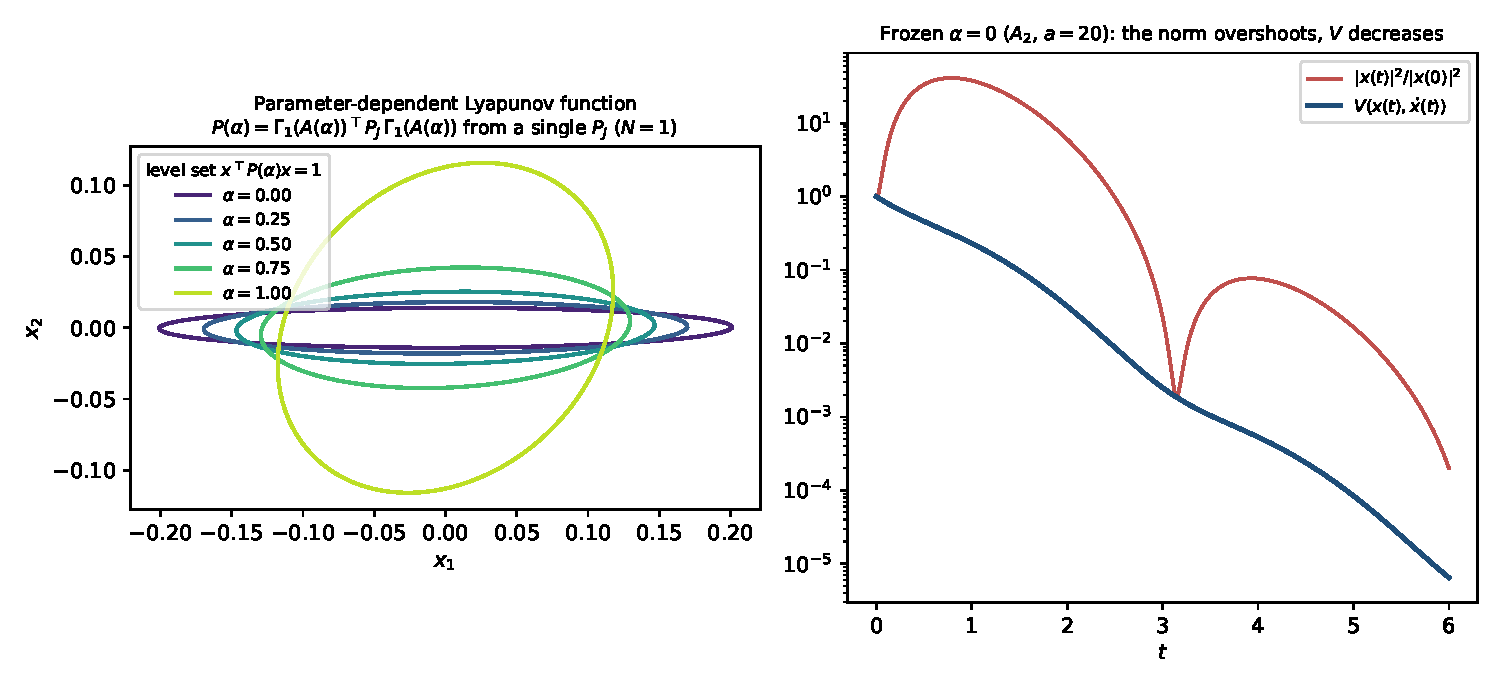
\includegraphics[width=\linewidth]{fig_polytope.pdf}
\caption{Polytope \eqref{eq:SN} with $a=20$. Left: level sets $x\tr P(\alpha)x=1$ of the parameter-dependent Lyapunov function generated by the level-$1$ certificate. Right: squared norm and $V(x,\dot x)$ along a trajectory of $\dot x=A_2x$.}\label{fig:polytope}
\end{figure}
\begin{figure}[t]\centering
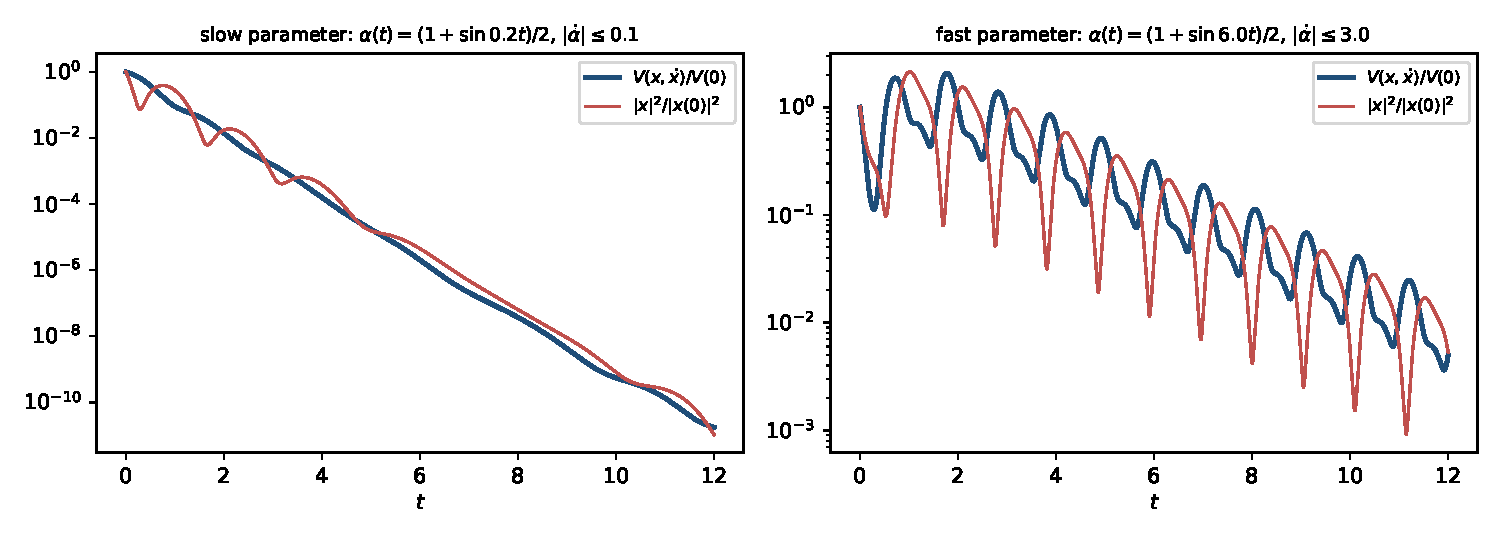
\includegraphics[width=\linewidth]{fig_polytope_tv.pdf}
\caption{Same certificate along solutions of $\dot x=A(\alpha(t))x$, $\alpha(t)=(1+\sin\omega t)/2$, for $\omega=0.2$ (left) and $\omega=6$ (right).}\label{fig:polytopetv}
\end{figure}

\subsection{A polytope that requires the second level}\label{sec:numlevel2}
The following three-vertex polytope in $\R^{3\times3}$ was obtained by taking similar copies $A_i=S_iJS_i^{-1}$ of the non-normal block $J$ with diagonal $-1$ and superdiagonal $b$, with random well-conditioned $S_i$, increasing $b$ until the polytope reaches the boundary of robust stability, and rescaling time:
\begin{equation}\label{eq:ex2}
A_1=\begin{pmatrix}-0.38&3.58&3.22\\2.32&1.62&1.65\\-3.21&-5.12&-4.72\end{pmatrix},\quad
A_2=\begin{pmatrix}1.63&1.03&1.12\\-10&-0.57&2.74\\4.46&-1.63&-4.54\end{pmatrix},\quad
A_3=\begin{pmatrix}-0.24&4.86&-1.98\\-1.24&-2.42&0.94\\-1.78&1.31&-0.83\end{pmatrix}.
\end{equation}
The eigenvalues of the vertices have real parts in $[-1.5,-0.98]$, and $\max_{\alpha\in\Delta_3}\max\operatorname{Re}\operatorname{eig}A(\alpha)=-0.024$ on a grid of $20\,301$ points of the simplex. For each level we computed the largest decrease margin $\gamma^*$ such that the decrease condition holds with $-\gamma^*I$ on the right-hand side, under the normalization $V\ge|x|^2$ on admissible jets and $\|\PP\|\le10^3$, both for the vertex LMIs \eqref{eq:vertex} and for the exact conditions \eqref{eq:robcond} imposed on a grid of $66$ values of $\alpha$; the latter are necessary conditions for any quadratic form in the $N$-jet. The results are $\gamma^*=-0.97$ (vertex) and $-8.19$ (grid) at level $0$, $\gamma^*=-0.38$ (vertex) and $-1.30$ (grid, confirmed by two solvers and unchanged with $\|\PP\|\le10^6$) at level $1$, and $\gamma^*=+3.61$ (vertex) at level $2$. Hence no quadratic form in $(x,\dot x)$ is a Lyapunov function for this family, whereas the level-$2$ vertex LMIs provide a certificate. For comparison, the same gridded conditions give $\gamma^*=-1.81$ for parameter-dependent functions affine in $\alpha$ and $\gamma^*=+5.33$ for homogeneous polynomial functions of degree $2$ in $\alpha$: the example illustrates the need for the second level of the hierarchy, and is consistent with the inclusion of the level-$1$ class in the degree-$2$ polynomial class (Remark~\ref{rem:slack}).

\subsection{A saturated feedback loop}\label{sec:numsat}
Consider \eqref{eq:sat} with
\begin{equation}\label{eq:satex}
A=\begin{pmatrix}0.3&1\\-1&0.3\end{pmatrix},\qquad B=\begin{pmatrix}0\\1\end{pmatrix},\qquad u_0=1,\qquad K\approx\begin{pmatrix}-12.86&-11.52\end{pmatrix},
\end{equation}
where $K$ is the LQR gain for the weights $Q=I$ and $R=0.01$. The open loop is an unstable focus, so that the region of attraction is bounded, and the high gain makes the linear region $\mathcal R_0$ a thin strip: most of the region of attraction lies in $\mathcal R_+\cup\mathcal R_-$. Proposition~\ref{prop:satLMI} was applied with $\varepsilon=10^{-4}$, a line search over logarithmic grids of $\lambda_e\in[10^{-2},10^{2}]$ and $\mu\in\{0\}\cup[10^{-2},10^{1.5}]$, and a bisection on $\beta$ for each pair. The best certificates found are $\beta=0.67$ for the quadratic function with the generalized sector condition ($\PP=\diag(P,0)$) and $\beta=1.09$ for the order-one jet function. Figure~\ref{fig:regional} compares the two estimates with the region of attraction computed by simulation on a grid of initial conditions. The jet estimate is made of three elliptic arcs glued continuously along the lines $|Kx|=u_0$ and covers about three times the area of the ellipsoidal estimate. Figure~\ref{fig:regionaltraj} shows $V$ along a trajectory starting on the boundary of the estimate: $V$ decreases monotonically, with a kink at each crossing of a saturation line, whereas the norm does not.

\begin{figure}[t]\centering
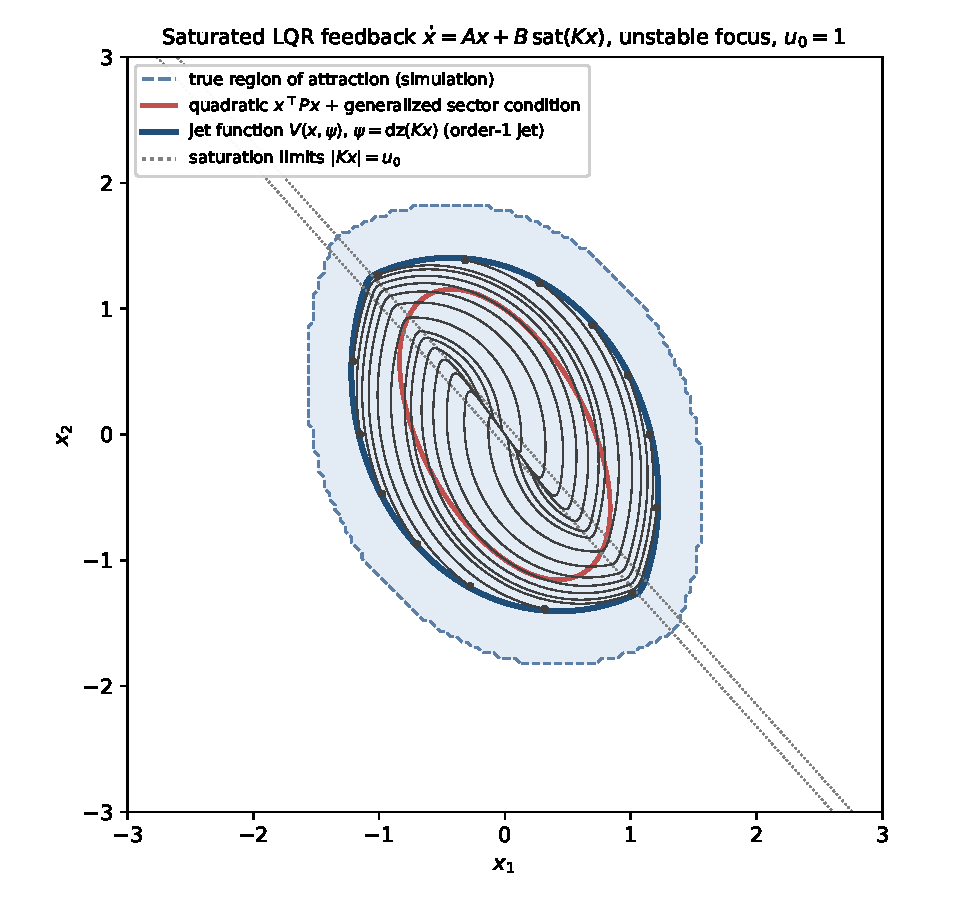
\includegraphics[width=0.72\linewidth]{fig_regional.pdf}
\caption{Saturated loop \eqref{eq:satex}: region of attraction (shaded, by simulation), ellipsoidal estimate with the generalized sector condition (red), order-one jet estimate $\{V(x,\dz(Kx))\le1\}$ (blue), and trajectories starting from its boundary.}\label{fig:regional}
\end{figure}
\begin{figure}[t]\centering
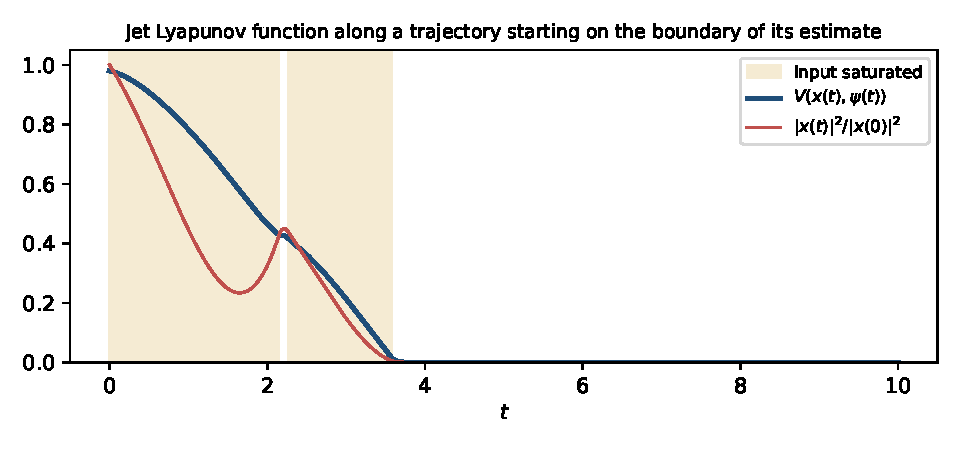
\includegraphics[width=0.8\linewidth]{fig_regional_traj.pdf}
\caption{Jet Lyapunov function and squared norm along a trajectory of Figure~\ref{fig:regional}; shaded intervals: saturated input.}\label{fig:regionaltraj}
\end{figure}

\section{Conclusions and open problems}\label{sec:conc}

Lyapunov functions on jets of trajectories formalize a widespread practice in LMI-based analysis. In the linear uncertain case they admit a converse theory built on a single universal quadratic form whose derivative obeys a system-independent identity; the theory extends to slowly varying parameters and to families of analytic nonlinear systems within the radius of convergence of the Lie series, and it adapts to the regional analysis of saturated systems, where the order of the jet is limited to one. The following questions are natural continuations.

\begin{problem}[constant multipliers]\label{pb:constG}
Is the vertex relaxation \eqref{eq:vertex}, with constant multipliers $G_0,G$, asymptotically exact as $N\to\infty$? In the proof of Theorem~\ref{thm:LTI}, the equality constraints are used only to identify $\tau_N(T)$ with $E_N(TA)x$, which suggests a multiplier depending polynomially on $A$ with a degree independent of $N$; if so, it could be absorbed by increasing $N$. The dual LMI techniques of \citet{Scherer2005,EbiharaBook2015} provide a way to test exactness level by level.
\end{problem}

\begin{problem}[rate-bounded converse]
Theorem~\ref{thm:tv} covers small rates. For a family that is robustly stable for all $w(\cdot)$ with $|\dot w|\le\delta_0$, does there exist a quadratic form in some jet that is a Lyapunov function for all rates below $\delta_0$? A route is Proposition~\ref{prop:PDLF}: apply a converse theorem for rate-bounded systems and use jet-identifiability to transport the resulting $W(x,w)$ to the jet space; the obstacle is the restriction to quadratic forms.
\end{problem}

\begin{problem}[Lur'e systems]
Establish a converse theorem for sector- and slope-restricted Lur'e systems, taking into account the conserved quantity of Remark~\ref{rem:lpv}, and relate the order of the jet to the order of Zames--Falb multipliers \citep{Carrasco2016}.
\end{problem}

\begin{problem}[beyond the radius of analyticity]\label{pb:NL}
For $f$ analytic and exponentially stable on a compact invariant set, does $\bigcup_N\mathcal Q_N(f)$ always contain a Lyapunov function? A negative answer would show that the predictive nature of jets is a genuine limitation; a positive one would require a mechanism different from Taylor truncation.
\end{problem}

\begin{problem}[non-smooth solutions]
For differential inclusions whose solutions are only absolutely continuous, what replaces the jet? One possibility is to restrict to $C^N$ selections and prove a density result; another is to define set-valued jets $\Jet^N_F(x)$ and study when $W(x)=\sup_{j\in\Jet^N_F(x)}V(j)$ is a Lyapunov function in the usual sense, in the spirit of \citet{MolchanovPyatnitskii1989,Blanchini1995}.
\end{problem}

\section*{Acknowledgements}
To be completed.

\bibliographystyle{elsarticle-harv}
\bibliography{refs}

\end{document}
